%---- Sample WMSU BSMATH BEAMER template ------
%---- Begin editing after PREAMBLE END at line 77------
%---- Created by: Christle Jude L. Maquilan - April 2022 --
%---- @jmaq03.jm@gmail.com -----

\documentclass[xcolor=dvipsnames,envcountsect]{beamer}

%------------------------------------------------
%------------------------------------------------
%------------------------------------------------
%------------------------------------------------
%------------------------------------------------
%----------▼▼▼▼▼ START PREAMBLE ▼▼▼▼▼----------

%-------- theme --------
\usetheme{Madrid}
%-------- packages to be used -------
\usepackage{amsmath,amsfonts,amssymb,amscd,amsthm}
\usepackage{graphicx,xcolor,comment}
\usepackage{mathrsfs}
\usepackage{multirow}
\usepackage{array}
\usepackage{hyperref}
\usepackage{multicol}
\usepackage{multimedia}
\usepackage{ragged2e}
\usepackage{siunitx}
\usepackage{tikz-feynman}
\usepackage{caption}
\usepackage[english]{babel}
\usepackage{rotating}
\usepackage{enumerate}
\usepackage{tikz}
\usepackage{bm}
\usepackage{csquotes}
\usepackage{mathtools}
\usepackage{relsize}
\usepackage{bbm}
\usepackage{pgfplots}
\usepackage{physics}
\usepackage{calligra}
\usepackage{csquotes}
\usepackage{tensor}
\usepackage[thicklines]{cancel}
\usepackage{tcolorbox}
\usepackage{pstricks}
%-------- color --------
\definecolor{blue2}{HTML}{045FB4}
\definecolor{green2}{HTML}{46C235}
\definecolor{red2}{HTML}{EE4848}
\definecolor{violet2}{HTML}{A647E5}
\definecolor{orange2}{HTML}{FF7425}
\definecolor{darkred}{HTML}{5C2020}
\definecolor{gray}{HTML}{303030}
\definecolor{yellow}{HTML}{f0be52}
\definecolor{lightdarkgold}{HTML}{EEBC1D}

%-------- set color of 'example block' to crimson theme --------
\usecolortheme[named=darkred]{structure}
\usecolortheme{sidebartab}
\usecolortheme{orchid}
\usecolortheme{whale}
\setbeamercolor{titlelike}{parent=structure, bg=structure, fg=white}
\setbeamercolor{section in toc}{fg= white}
\setbeamercolor{subsection in toc}{fg= white}
%\setbeamercolor*{sidebar}{fg=red2,bg=gray!15!white}

\setbeamercolor{item projected}{bg=yellow, fg = white}
\setbeamertemplate{enumerate items}[default]
\setbeamertemplate{navigation symbols}{}
\setbeamercolor{local structure}{fg=yellow}

\setbeamercolor{alerted text}{fg=white}
\setbeamercolor{block title}{bg = blue2}
\setbeamercolor{block title alerted}{bg=red2}
\setbeamercolor{block title example}{bg=green2}
\setbeamercolor{background canvas}{bg=gray}
\setbeamercolor{normal text}{bg=gray,fg=white}
%-------- font ---
\usefonttheme[stillsansseriftext]{structurebold}
\setbeamercovered{transparent}
%-------- misc structure --------
\useoutertheme[footline=authortitle,subsection=false]{miniframes}
\useinnertheme{rounded}
\addtobeamertemplate{block begin}{}{\justifying}
\newtheorem{remark}[theorem]{Remark}
\renewcommand{\indent}{\hspace*{2em}}
\setbeamertemplate{theorems}[numbered]
\setbeamertemplate{caption}[numbered]
\usepackage[justification=centering]{caption}
\renewcommand{\qedsymbol}{$\blacksquare$}

\newcommand*{\Scale}[2][4]{\scalebox{#1}{$#2$}}%
\usepackage[bigfiles]{pdfbase}
\ExplSyntaxOn
\NewDocumentCommand\embedvideo{smm}{
	\group_begin:
	\leavevmode
	\tl_if_exist:cTF{file_\file_mdfive_hash:n{#3}}{
		\tl_set_eq:Nc\video{file_\file_mdfive_hash:n{#3}}
	}{
		\IfFileExists{#3}{}{\GenericError{}{File~`#3'~not~found}{}{}}
		\pbs_pdfobj:nnn{}{fstream}{{}{#3}}
		\pbs_pdfobj:nnn{}{dict}{
			/Type/Filespec/F~(#3)/UF~(#3)
			/EF~<</F~\pbs_pdflastobj:>>
		}
		\tl_set:Nx\video{\pbs_pdflastobj:}
		\tl_gset_eq:cN{file_\file_mdfive_hash:n{#3}}\video
	}
	%
	\pbs_pdfobj:nnn{}{dict}{
		/Type/RichMediaInstance/Subtype/Video
		/Asset~\video
		/Params~<</FlashVars (
		source=#3&
		skin=SkinOverAllNoFullNoCaption.swf&
		skinAutoHide=true&
		skinBackgroundColor=0x5F5F5F&
		skinBackgroundAlpha=0.75
		)>>
	}
	%
	\pbs_pdfobj:nnn{}{dict}{
		/Type/RichMediaConfiguration/Subtype/Video
		/Instances~[\pbs_pdflastobj:]
	}
	%
	\pbs_pdfobj:nnn{}{dict}{
		/Type/RichMediaContent
		/Assets~<<
		/Names~[(#3)~\video]
		>>
		/Configurations~[\pbs_pdflastobj:]
	}
	\tl_set:Nx\rmcontent{\pbs_pdflastobj:}
	%
	\pbs_pdfobj:nnn{}{dict}{
		/Activation~<<
		/Condition/\IfBooleanTF{#1}{PV}{XA}
		/Presentation~<</Style/Embedded>>
		>>
		/Deactivation~<</Condition/PI>>
	}
	%
	\hbox_set:Nn\l_tmpa_box{#2}
	\tl_set:Nx\l_box_wd_tl{\dim_use:N\box_wd:N\l_tmpa_box}
	\tl_set:Nx\l_box_ht_tl{\dim_use:N\box_ht:N\l_tmpa_box}
	\tl_set:Nx\l_box_dp_tl{\dim_use:N\box_dp:N\l_tmpa_box}
	\pbs_pdfxform:nnnnn{1}{1}{}{}{\l_tmpa_box}
	%
	\pbs_pdfannot:nnnn{\l_box_wd_tl}{\l_box_ht_tl}{\l_box_dp_tl}{
		/Subtype/RichMedia
		/BS~<</W~0/S/S>>
		/Contents~(embedded~video~file:#3)
		/NM~(rma:#3)
		/AP~<</N~\pbs_pdflastxform:>>
		/RichMediaSettings~\pbs_pdflastobj:
		/RichMediaContent~\rmcontent
	}
	\phantom{#2}
	\group_end:
}
\ExplSyntaxOff


%-------- for bibliography -----------------
\usepackage[backend=biber, bibstyle=nature, sorting=nty, citestyle=numeric-comp]{biblatex} %Custom bibliography
\addbibresource{bib.bib} %Load references

%-------- WMSU Backgound -------------------
%\usebackgroundtemplate{%
%	\tikz[overlay,remember picture] \node[opacity=0.02, at=(current page.center)] {
%		
\includegraphics[height=4.5in,width=4.5in]{Figures/logo.pdf}};
%}

%----------▲▲▲▲▲ PREAMBLE END ▲▲▲▲▲----------
%------------------------------------------------
%------------------------------------------------
%------------------------------------------------
%------------------------------------------------
%------------------------------------------------

%---------START EDITING HERE---------------------
\title[Ultralight Dark Matter]{Ultralight Dark Matter}

\author[Bruno Parracho (97855)]{\textbf{Bruno F. Parracho}}

\institute[University of Aveiro] {\emph{Superviser: }\textbf{António Morais, Ph.D.}\\[1em]
	Department of Physics\\University of Aveiro\\[1em]

\includegraphics[scale=.8]{./Figures/logo.pdf}}

\date[July 28, 2022]{\footnotesize Project - Defense - \textbf{July 28, 2022}}
%--------- START DOCUMENT ------------------

\begin{document}
    
    \frame{\titlepage}
    
    \begin{frame}{Summary}
        \tableofcontents
    \end{frame}
    
    \section{Missing matter}

\begin{frame}
    
    \begin{figure}
         \centering
         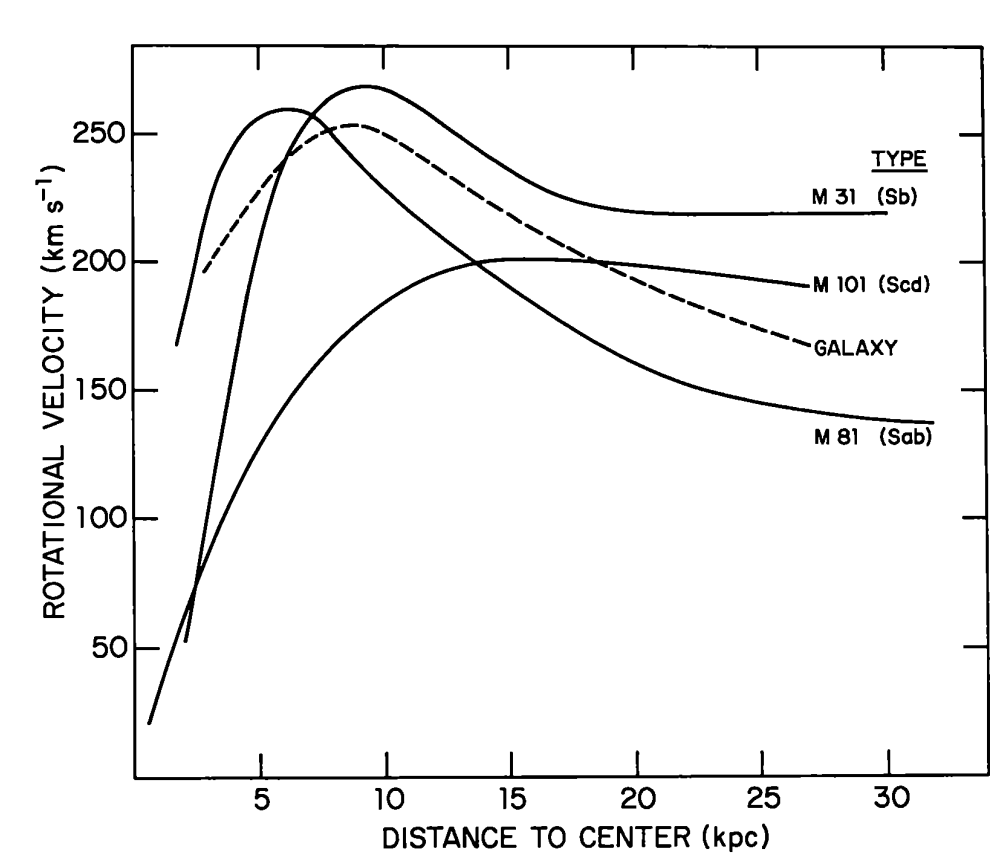
\includegraphics[width=.7\textwidth]{Figures/rotation-curves.png}
        \caption{Rotation curves of some galaxies REFERENCIA}
        \label{fig:rot}
    \end{figure}
    
\end{frame}

\begin{frame}{Models and recipes}
\begin{columns}
\begin{column}{0.5\textwidth}
Properties:
    \begin{itemize}
        \item Neutral
        \item Stable
        \item Cold
        \item Weakly interacting
    \end{itemize}
    \bigskip
Candidates:
    \begin{itemize}
        \item WIMPs
        \item FIMPs
        \item \textcolor{yellow}{Ultralight scalars}
        \textcolor{yellow}{$m_\theta \sim \mathcal{O}(10^{-10}-10^{-20})$ \si{\eV}}
    \end{itemize}
\end{column}
\begin{column}{0.5\textwidth}
Ways to produce:
\begin{itemize}
    \item Freeze-Out
    \item Freeze-In
    \item Cosmic strings
    \item Domain Walls
    \item \textcolor{yellow}{Misalignment mechanism}
\end{itemize}
\end{column}
\end{columns}
\end{frame}
    \section{Ultralight Model}
\frame{\sectionpage}

\begin{frame}{Eletroweak theory}
\begin{block}{Higgs Potential}
\begin{equation}
    V_0(H)=\mu_{H}^{2}H^{\dag}H+\frac{1}{2}\lambda_H(H^{\dag}H)^2
\end{equation}
\end{block}
\begin{block}{Scalar Potential
\cite{Freitas_2021}}
\begin{equation}
    V(H,\phi)=V_0(H)+\mu_\phi^2\phi^*\phi+\frac{1}{2}\lambda_\phi|\phi^*\phi|^2+\lambda_{H\phi}H^{\dag}H\phi^*\phi
\end{equation}
\end{block}

\end{frame}
\begin{frame}
    \pause
    \begin{block}{Soft breaking potential}
    \begin{equation}
        V(H,\phi)\rightarrow V(H,\phi)+\dfrac{\mu_s^2}{2}\left(\phi´^2+\phi^{*2}\right)
    \end{equation}
    \end{block}
    \pause
    The scalar takes the form of
    \bigskip
    \begin{equation}
        \phi=\dfrac{1}{\sqrt{2}}(\sigma+v_\sigma)e^{i\theta/v_\sigma}
    \end{equation}
    \pause
    The mass of the pNGB reads as
    \begin{equation}
	m^2_\theta=-2\mu_s^2
    \end{equation}
\end{frame}
%\begin{frame}
%    Basis change:
%    \begin{equation}
%	\left(\begin{array}{l}
%		h_1 \\
%		h_2 \\
%		\theta 
	%\end{array}\right)=\left(\begin{arr%ay}{lll}
		%\cos(\alpha) & \sin(\alpha) & 0 %\\
		%-\sin(\alpha) & \cos(\alpha) & %0 \\
%		0 & 0 & 1
	%\end{array}\right)\left(\begin{arra%y}{l}
	%h \\
	%\sigma \\
	%\theta 
    %\end{array}\right)
    %\end{equation}
    %\begin{equation}
	%m^2=U^\dag M^2 U = %\left(\begin{array}{ccc}
%		m^2_{h_1} & 0 & 0 \\%
%		0 & m^2_{h_2} & 0 \\
%		0 & 0 & m^2_{\theta}
	%\end{array}\right)\,,
    %\end{equation}
    %\bigskip
    %\pause
    %Masses of the physical particles% %are
%    \begin{equation}
%    \label{masses}
%	\begin{array}{c}
	%	m^2_{h_{1,2}}=\frac{1}{2}\left[%v_h^2\lambda_H+v_\sigma^2\lambd%a_\phi\mp\sqrt{v_h^4\lambda_H^2%+v_\sigma^4\lambda_\phi^2+2v_h^%2v_\sigma^2(2\lambda_{H\phi}^2-%\lambda_H\lambda_\phi)}\right] %\\[10pt]
%		m^2_\theta=-2\mu_s^2\,,
%	\end{array}
%\end{equation}
%\end{frame}
%

    
    \section{Interaction Rate}

\begin{frame}{Thermal bath}
\begin{columns}
    \begin{column}{0.5\textwidth}
    Interaction rate and Hubble constant:
        \begin{align}
	    \label{eq}
	    \begin{array}{ll}
		\Gamma > H \quad (coupled) \\
		\Gamma < H \quad (decoupled)\,,
	    \end{array}
        \end{align}
    \end{column}
    \begin{column}{0.5\textwidth}
\begin{center}
	\embedvideo*{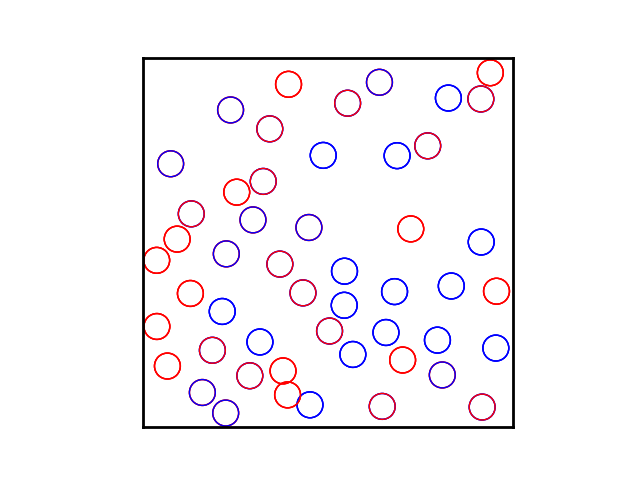
\includegraphics[width=\textwidth]{Figures/oie_transparent}}{collision.mp4}
\end{center}
    \end{column}
\end{columns}
\end{frame}
    
\begin{frame}
    \pause
\begin{block}{Interaction rate \cite{kolb}}
    \begin{equation}
	\Gamma=n\langle \sigma v \rangle =\frac{g}{16m^2\pi^2K_2(m/T)}\int_{4m^2}^\infty\sigma(s-4m^2)\sqrt{s}K_1\left(\frac{\sqrt{s}}{T}\right)ds\,.
    \end{equation}
\end{block}
\bigskip
\begin{itemize}
 \pause
 \item $|\overline{M}|^2_{1 + 2 \rightarrow 3 + 4}=|\overline{M}|^2_{3 + 4 \rightarrow 1 + 2}=|\overline{M}|^2$ \cite{kolb}
 \end{itemize}
\end{frame}
\begin{frame}{Amplitude}
Coupling terms ($\theta+\theta\rightarrow SM+\overline{SM}$): 
    \begin{align}
	\label{couplingterms}
	\begin{array}{ll}
	&\lambda_{\theta\theta h_i}=\dfrac{m_{h_1}^2}{v_\sigma}U_{2i}\,,\\	[8pt]
	&\lambda_{h_i SM SM}=U_{1i}g_{SM}\,.
	\end{array}
    \end{align}
    \pause
    Feynman diagram (s-channel):
    \begin{columns}
    \begin{column}{0.5\textwidth}
    \begin{center}
    \feynmandiagram[horizontal=a to b]{
    i1 [particle=\(\theta\)] --[scalar] a --[scalar] i2 [particle=\(\theta\)] ,
    a -- [boson,edge label=\(h_{1,2}\)] b, 
    f1 [particle=\(SM\)]  --[fermion] b -- [fermion]  f2[particle=\(\overline{SM}\)], 
    };
    \end{center}
    \end{column}
    \begin{column}{0.5\textwidth}
    \pause
    \begin{center}
    \begin{itemize}
        \item CalcHEP
    \end{itemize}
    \end{center}
    \end{column}
    \end{columns}
\end{frame}
\begin{frame}
    \begin{figure}
         \centering 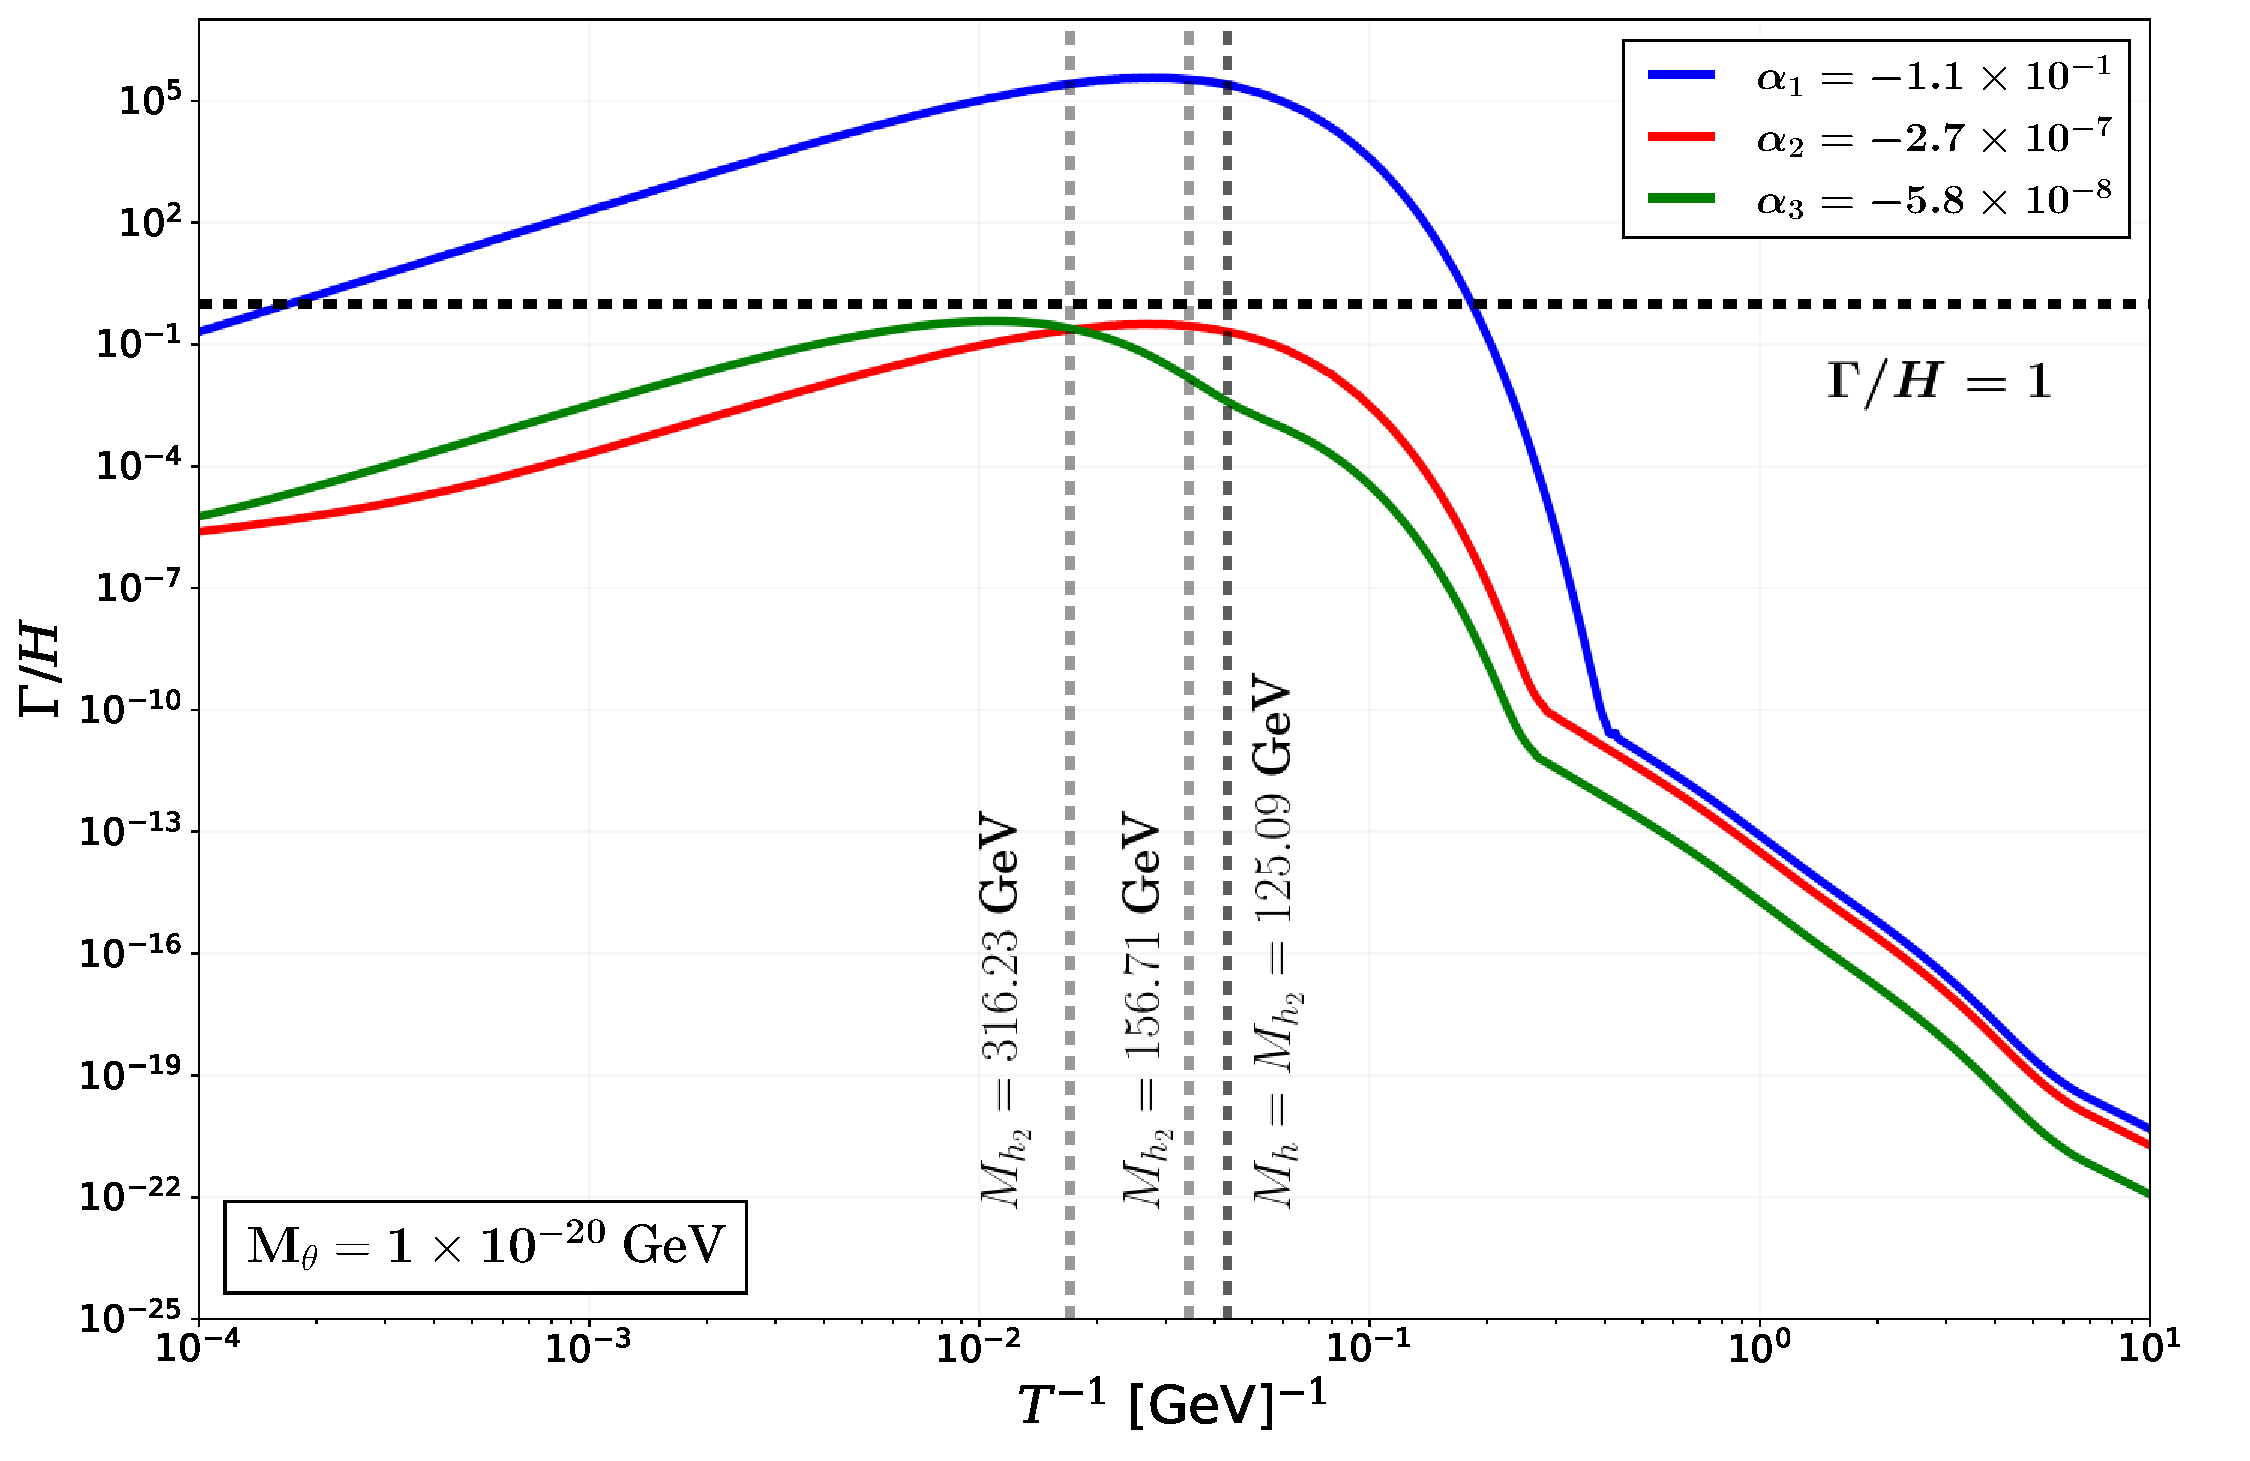
\includegraphics[width=.8\textwidth]{Figures/ratedm_equal.pdf}
        \caption{Rate of interaction divided by the Hubble constant assuming $m_h = m_{h_2}$ for $\lambda_H\sim0.26$, $\lambda_{H\phi}=2\times10^{-8}$ and $\lambda_\phi=0.1$}
        \label{fig:rot}
    \end{figure}
\end{frame}
\begin{frame}
        \begin{figure}
         \centering
         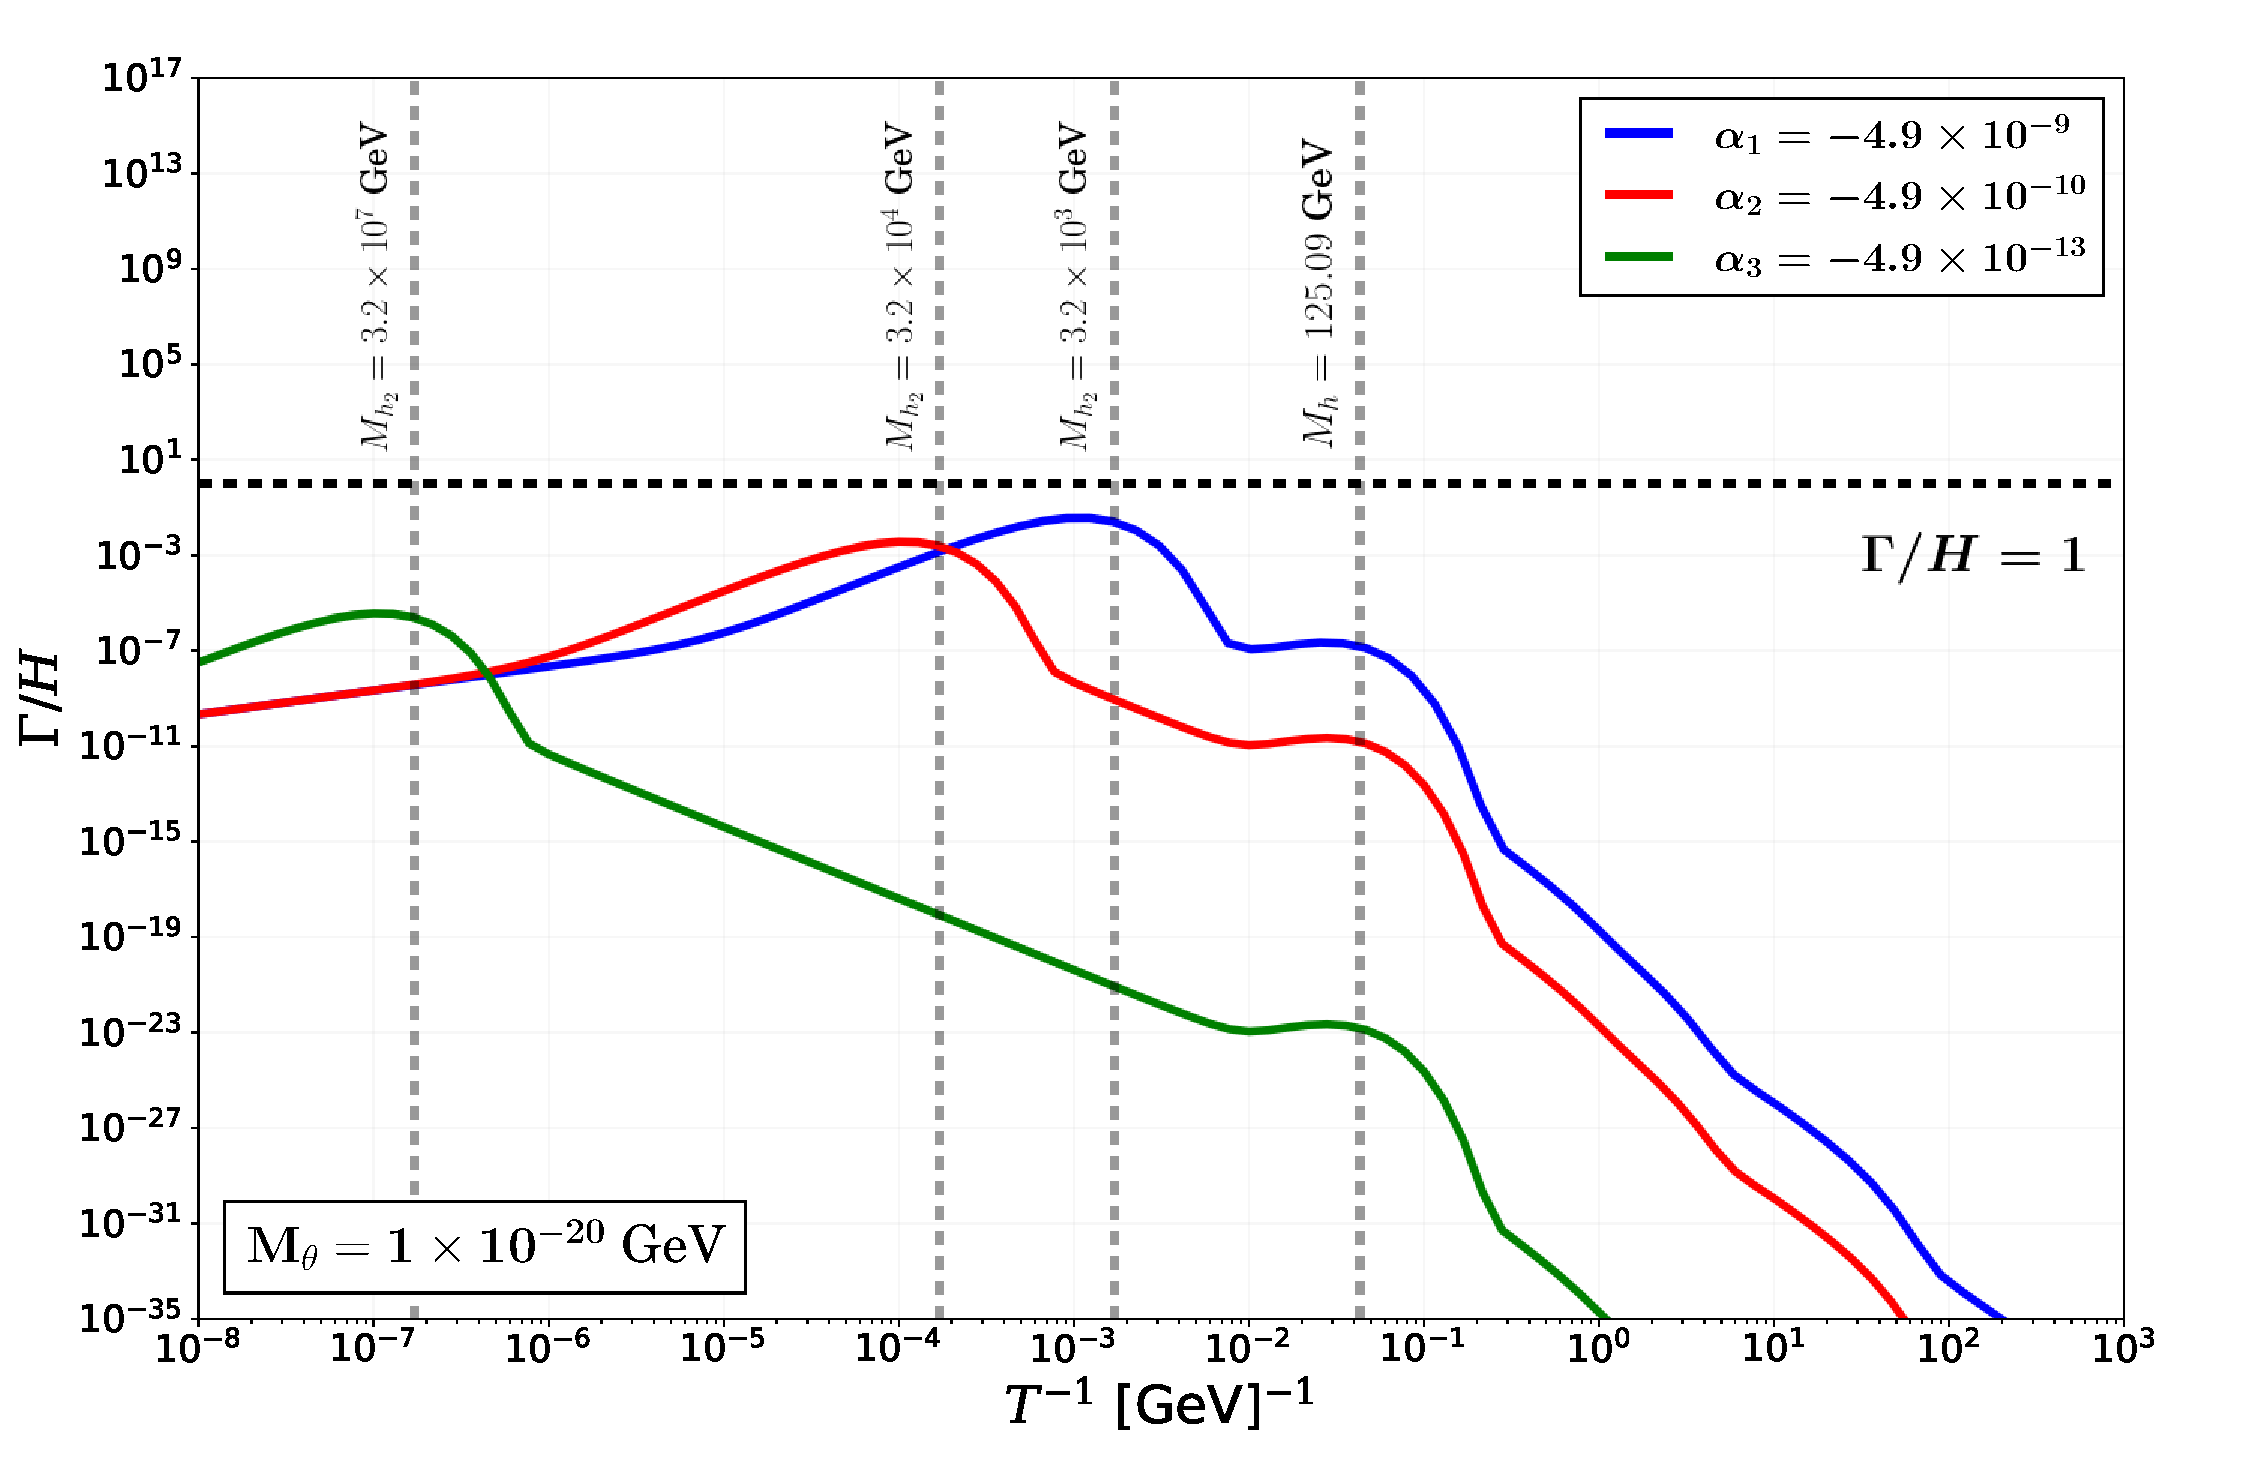
\includegraphics[width=.8\textwidth]{Figures/ratedm_greater.pdf}
        \caption{Rate of interaction divided by the Hubble constant assuming $m_h < m_{h_2}$ for $\lambda_H\sim0.26$, $\lambda_{H\phi}=2\times10^{-8}$ and $\lambda_\phi=0.1$}
        \label{fig:rot}
    \end{figure}
\end{frame}
\begin{frame}
        \begin{figure}
         \centering
         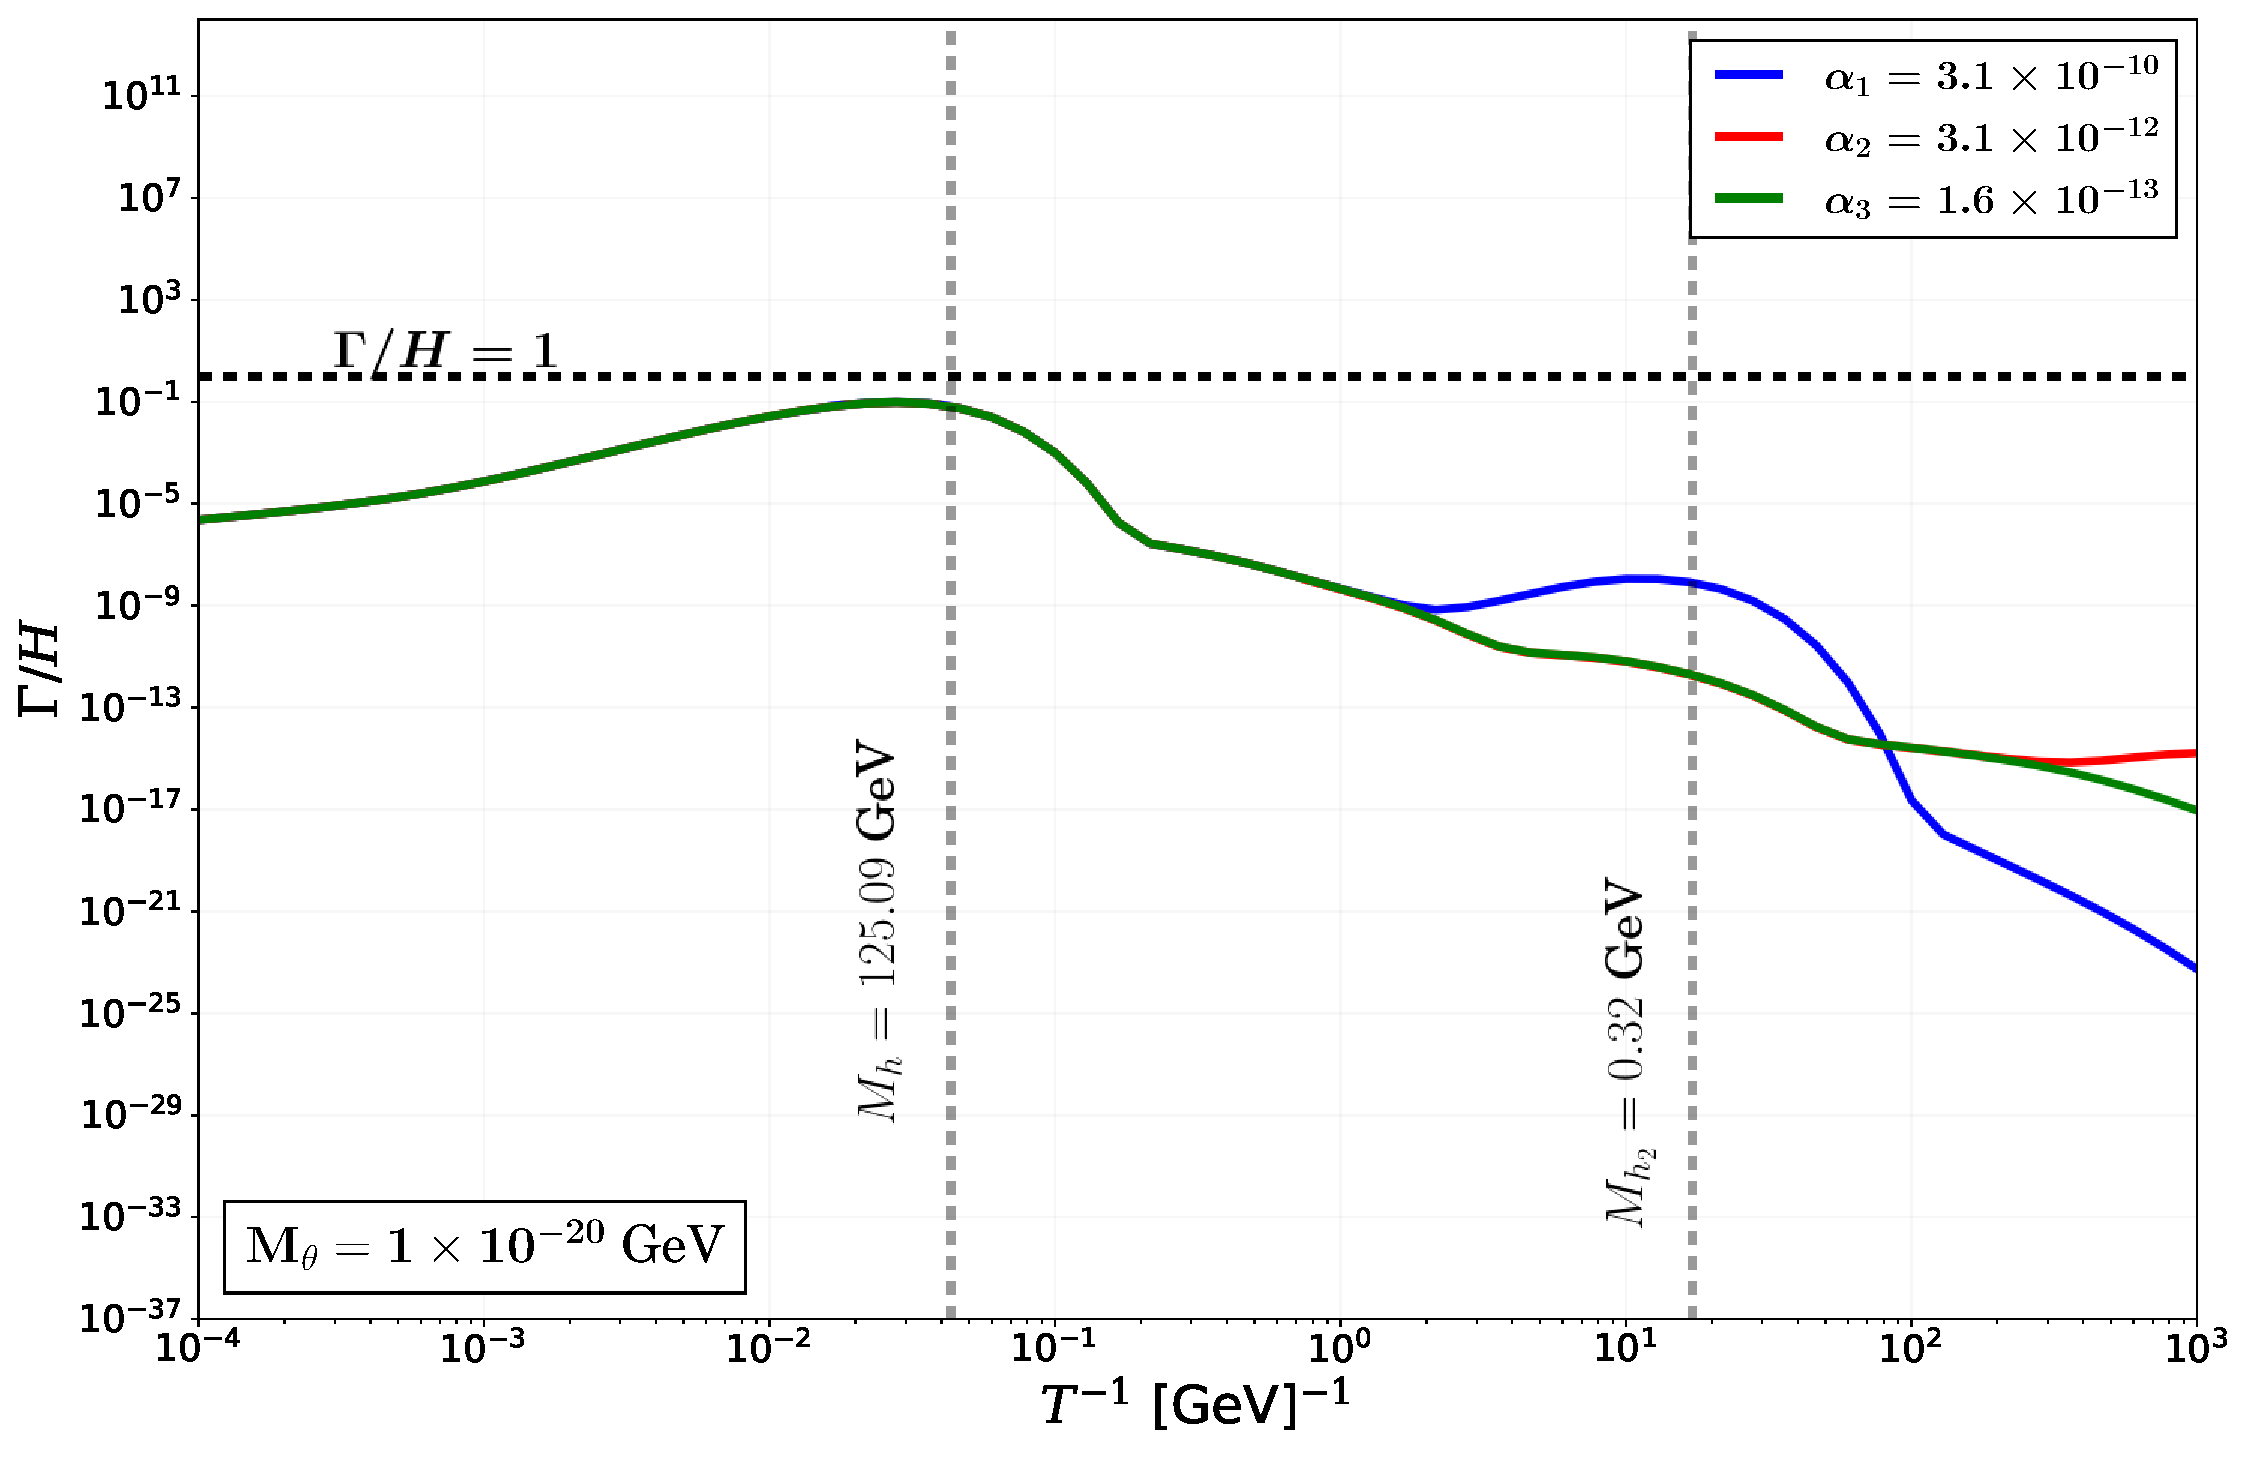
\includegraphics[width=.8\textwidth]{Figures/ratedm_lesser.pdf}
        \caption{Rate of interaction divided by the Hubble constant assuming $m_h > m_{h_2}$ for $\lambda_H\sim0.26$, $\lambda_{H\phi}=2\times10^{-8}$ and $\lambda_\phi=0.1$}
        \label{fig:rot}
    \end{figure}
\end{frame}
    
    \section{Misalignment Mechanism}

\begin{frame}{Misalignment Mechanism}
\begin{block}{Aproximation of the soft potential}
    \begin{equation}
    V_{\textrm{soft}}(\Theta)\simeq \frac{m_\theta^2}{2}\left(\frac{v_\sigma}{2}\right)^2\Theta^2, \textrm{ where } \Theta=2\theta/v_\sigma
\end{equation}
\end{block}
The energy density is given by
\begin{equation}
    \rho_\theta=-T^0_0=\left(\dfrac{v_\sigma}{2}\right)^2\left[\dfrac{\dot{\Theta}^2}{2}+\dfrac{m_\theta^2}{2}\Theta^2\right]\,,
\end{equation}
\begin{block}{Continuity equation}
\begin{equation}
\dot{\rho}+3H(\rho+P)=0
\end{equation}
\end{block}
For Matter ($P=0$):
\begin{equation}
    \rho(a) \propto a^{-3}
\end{equation}
\end{frame}

\begin{frame}
\begin{block}{Equation of Motion}
    \begin{equation}
    \label{motion}
    \ddot{\Theta}^2+3H\dot{\Theta}+m_\theta^2\Theta=0\,.
\end{equation}
\end{block}
Radiation era: $a\propto \sqrt{t} \Rightarrow H=1/t$
 \begin{figure}
         \centering
         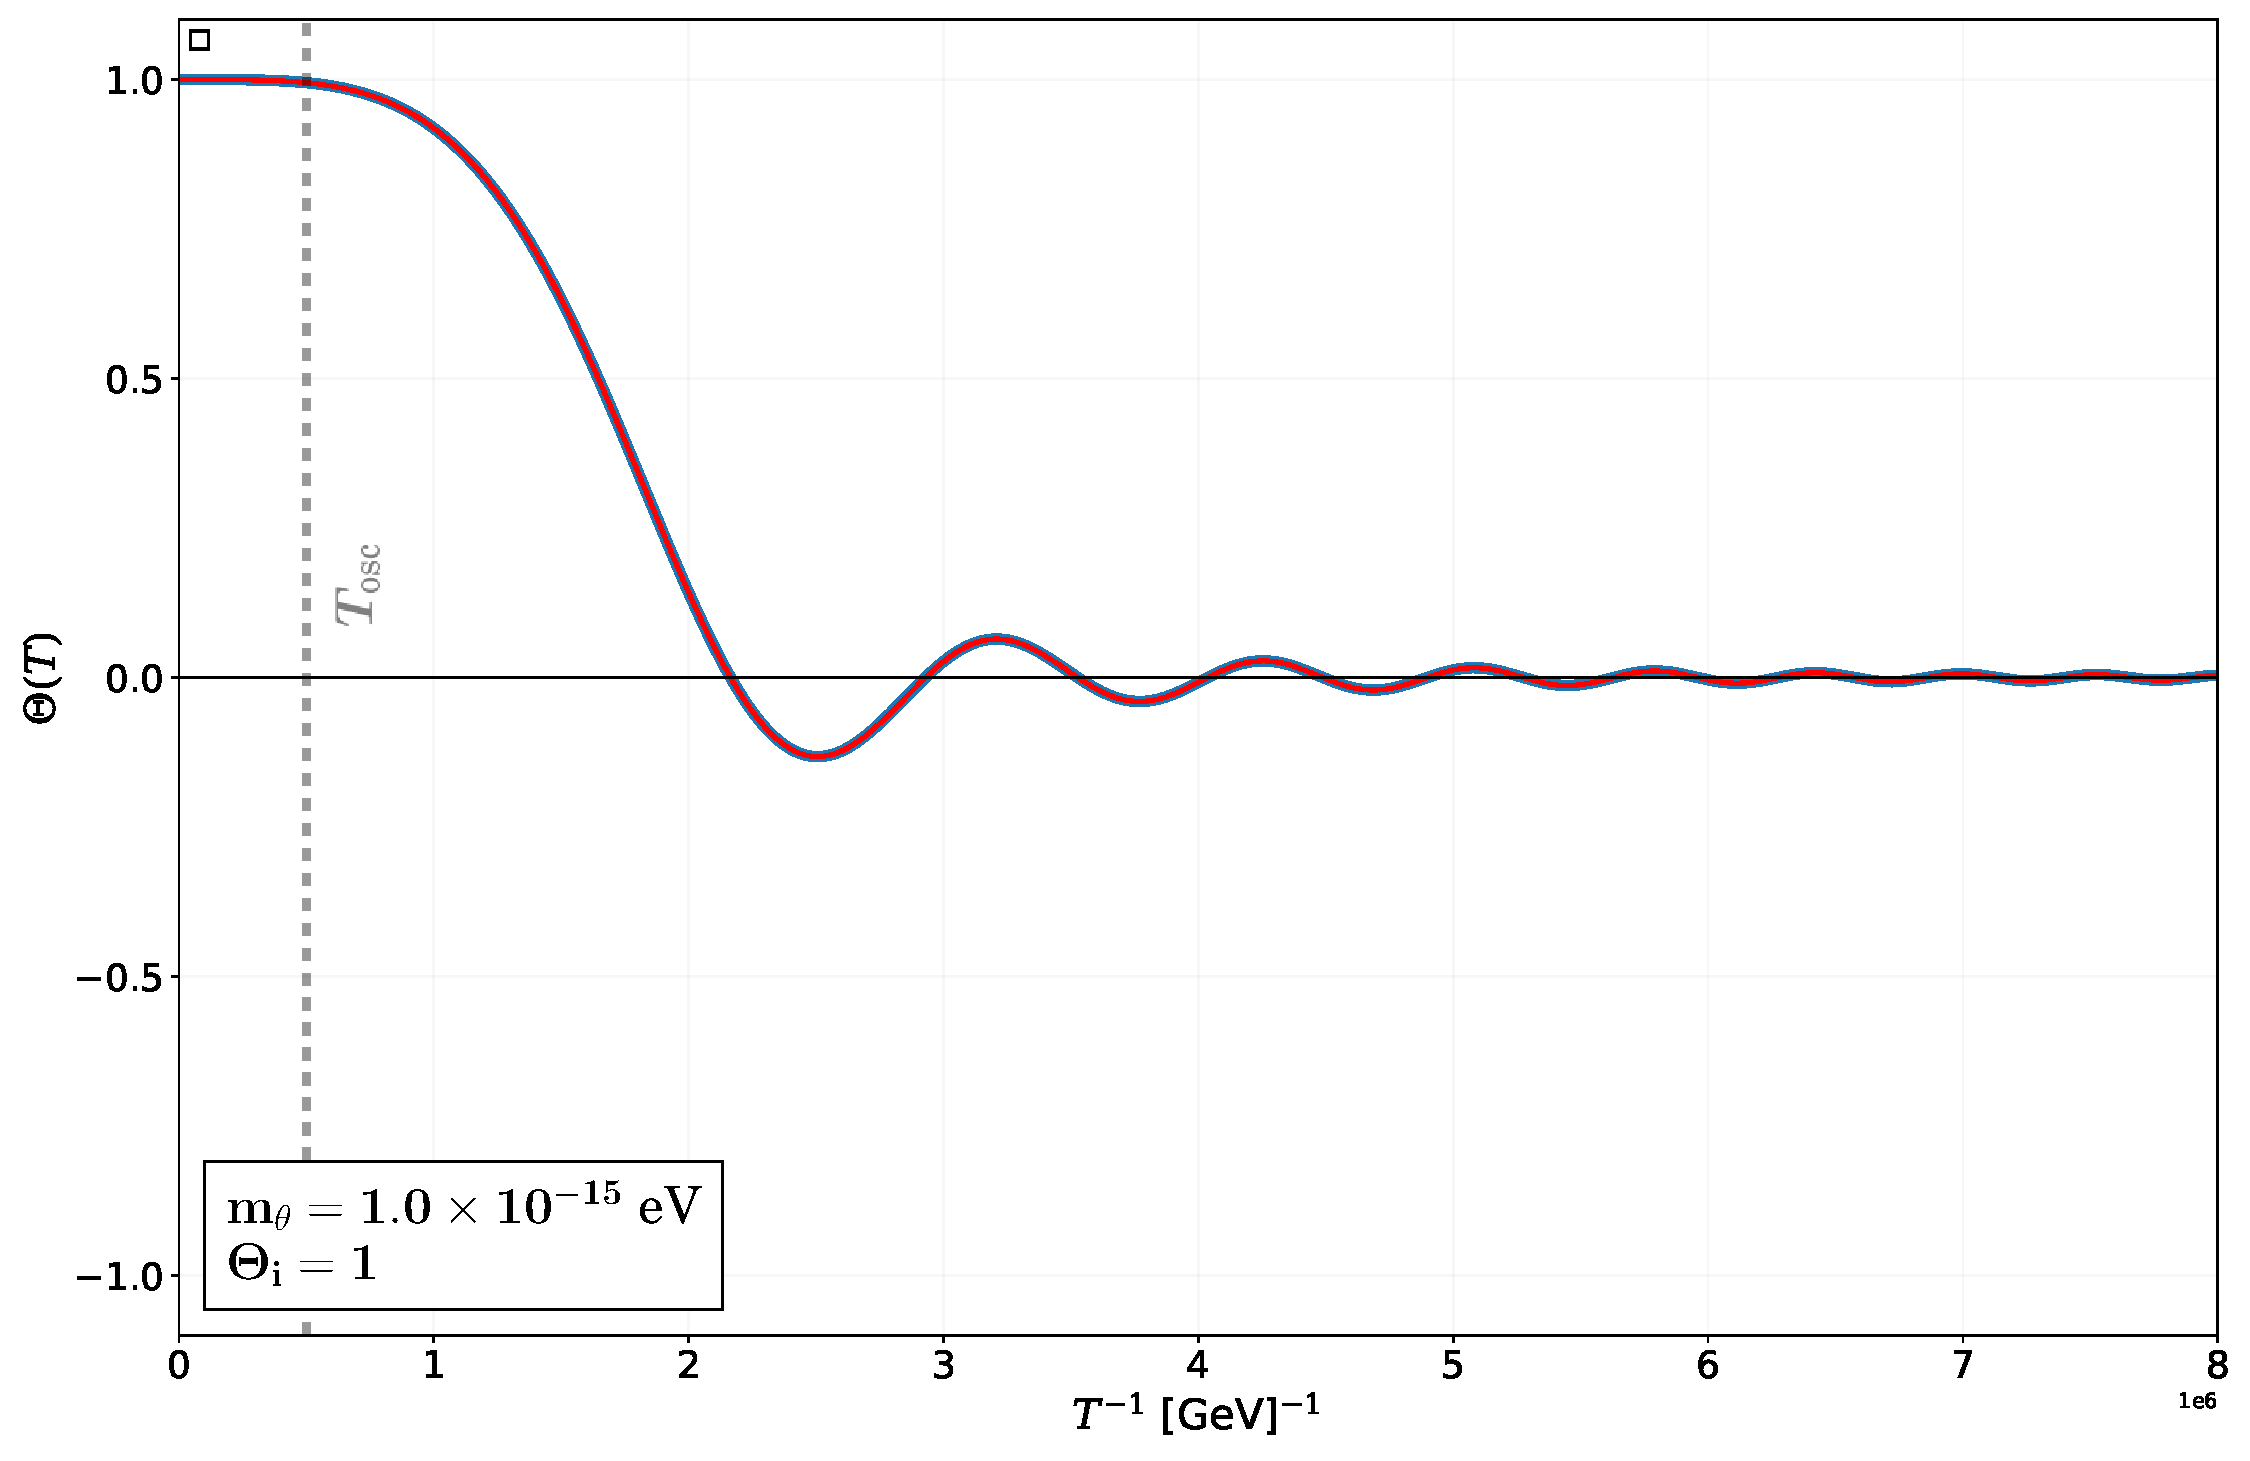
\includegraphics[width=.7\textwidth]{Figures/motion.pdf}
        \caption{Solution of the equation of motion}
        \label{fig:rot}
    \end{figure}
\end{frame}

\begin{frame}{Relic Density of pNGB}
    \[\Scale[0.7]{\Omega^0_\theta h^2=0.11\left(\dfrac{m_\theta}{10^{-14}\si{\eV}}\right)^{1/2}\left(\dfrac{v_\sigma}{\sqrt{50}\times10^{17}\si{G\eV}}\right)^{2}\left(\dfrac{\Theta_\textrm{osc}}{10^{-3}}\right)^{2}\left(\dfrac{3.91}{g_{*s}(T_\textrm{osc})}\right)\left(\dfrac{g_*(T_\textrm{osc})}{3.36}\right)^{3/4}}\]
 %
	\begin{figure}[H]
	\centering
	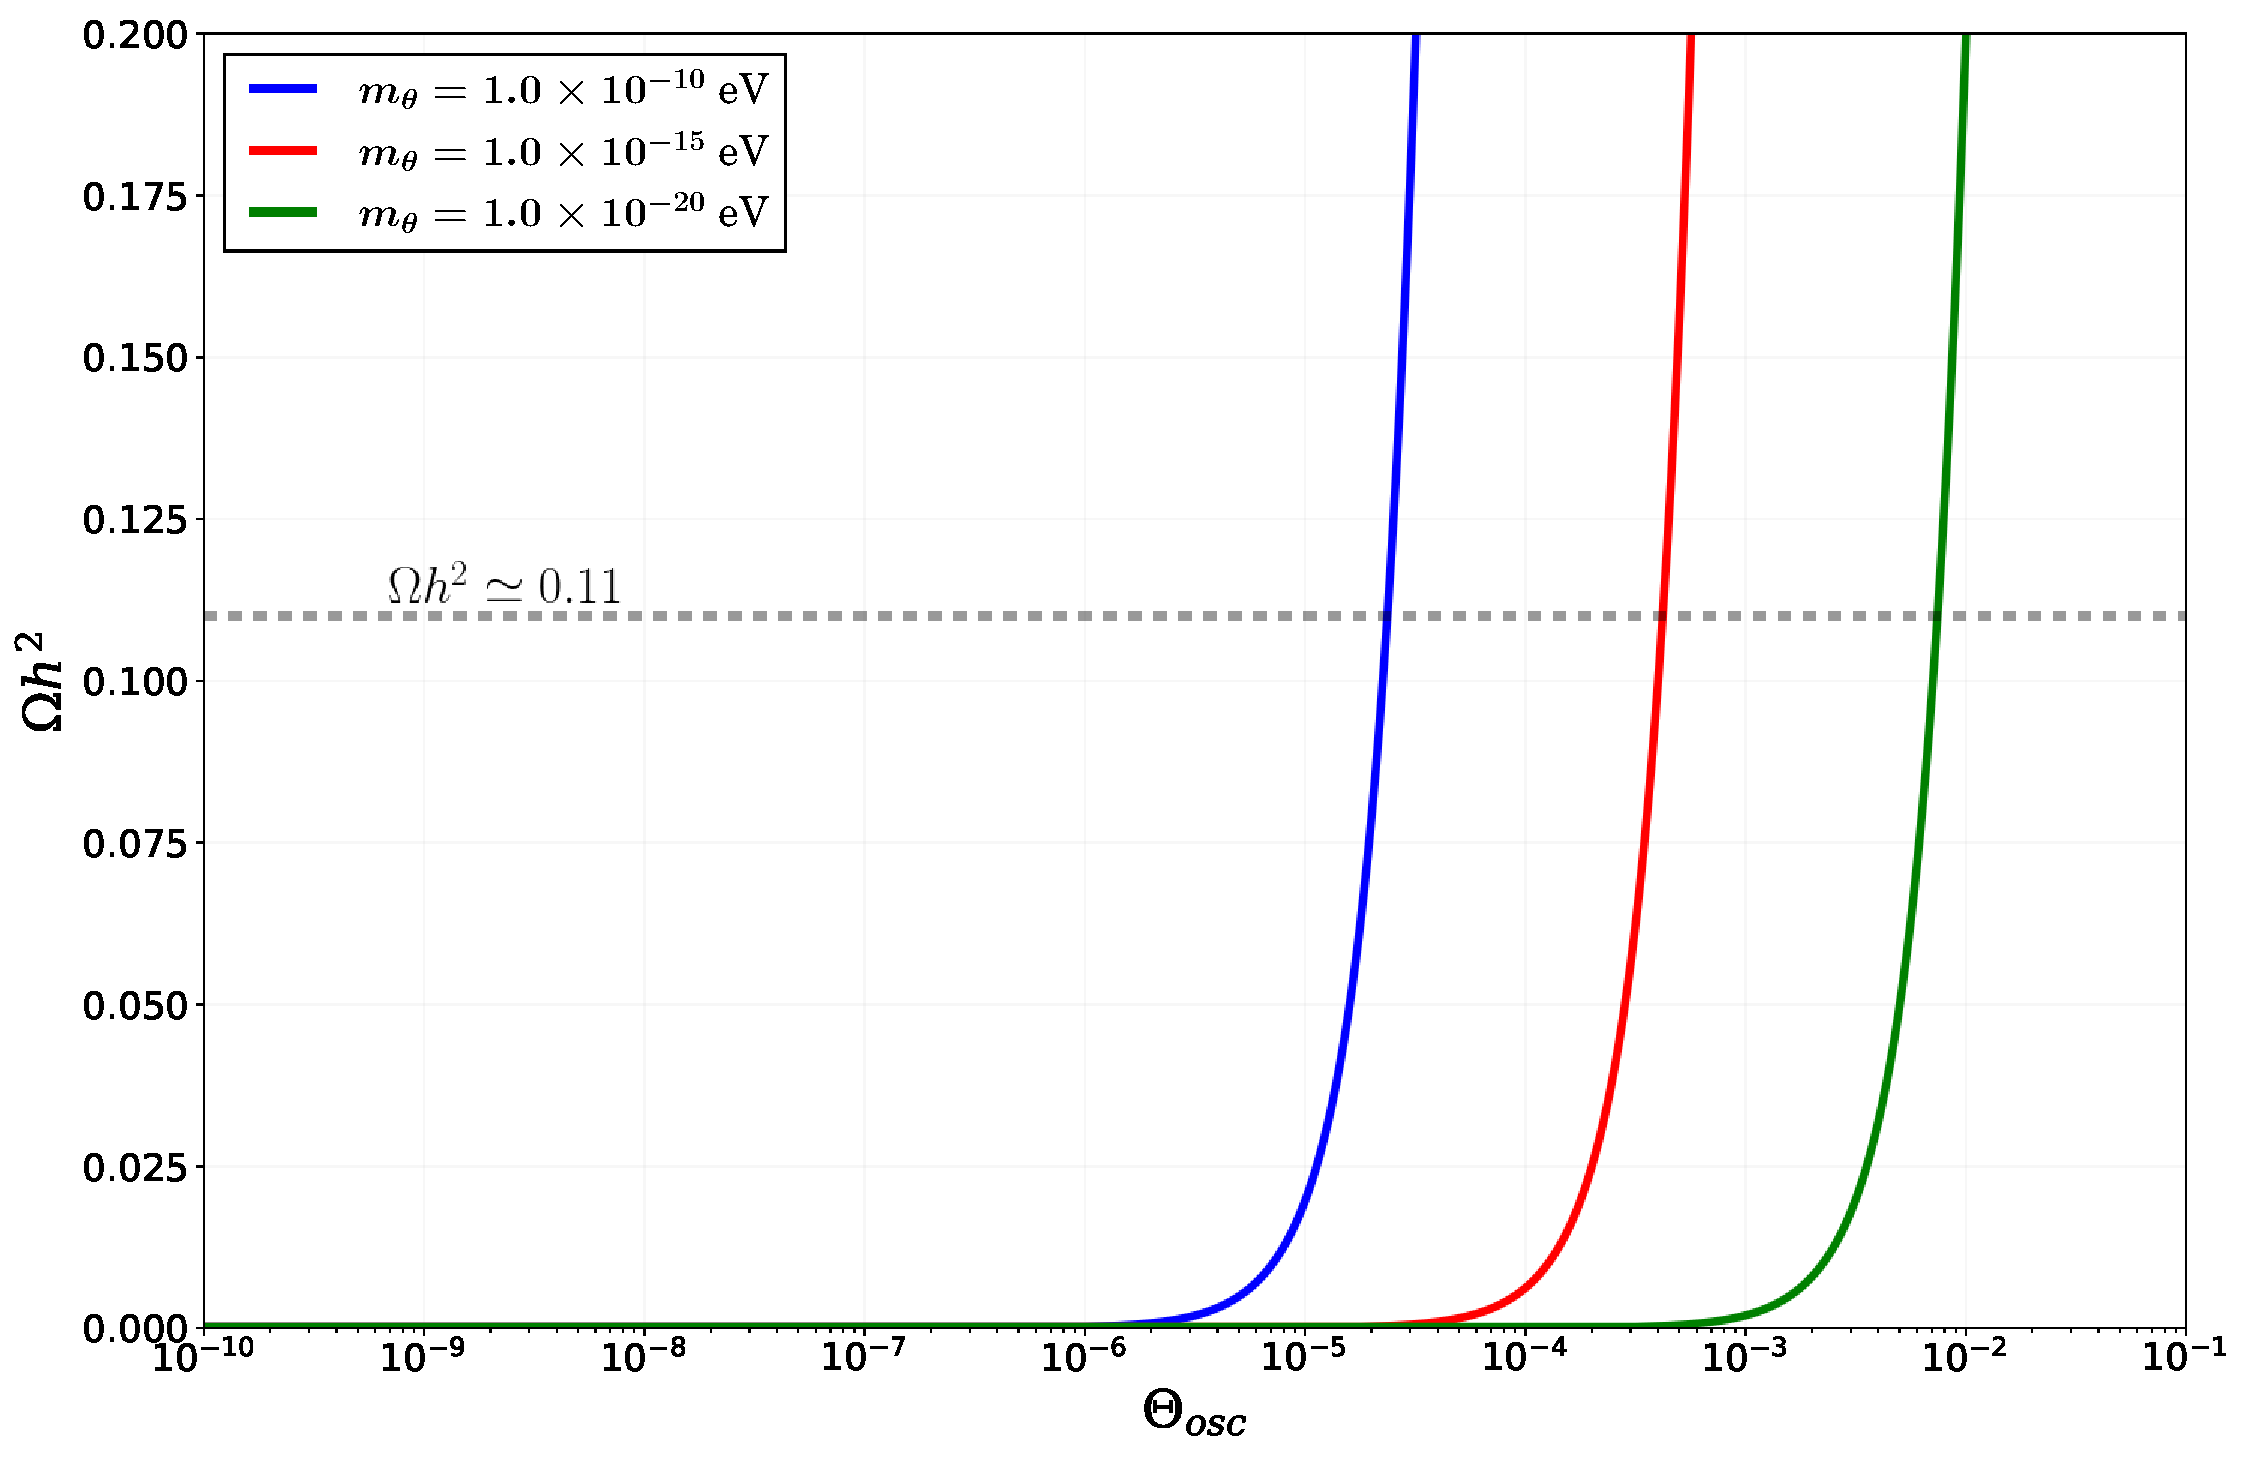
\includegraphics[width=0.6\linewidth]{Figures/relic_density.pdf}
	\caption{Relic density change with the initial Misalignment angle $\Theta_\textrm{osc}$, with $v_\sigma=3\times 10^{18}$, for various values of $m_\theta$\,.}
	\label{fig:relicdesity}
	\end{figure}
\end{frame}
 

    
    \section*{References} %You can remove this if you do not want to use it
    	\begin{frame}{References}
            \printbibliography
    	\end{frame}

    \section{}
    \begin{frame}{}
        \centering
            \Huge\bfseries
        \textcolor{yellow}{Thank you!!!}
    \end{frame}
\end{document}